\chapter{Systemarchitektur}
\label{chap:imp}
In folgendem Kapitel wird die Implementierung des, in Kapitel \ref{chap:ein} beschriebenen, Videoanalysesystems behandelt. Dabei wird zunächst in Abschnitt \ref{sec:mess} der Aufbau des Systems und die Funktion der Bildauswertungssoftware als Teil der gesamten Systemarchitektur erklärt. Im Abschnitt \ref{sec:sig} wird die Umsetzung der Eingangsgrößen (Bilder als Sensorsignale) in Messgrößen wie Personenzahl, -fluss oder -dichte in bestimmten Bildausschnitten beschrieben. Die Umsetzung erfolgt auf Basis der, in Kapitel \ref{chap:grund} beschriebenen, Grundlagen. Weiterhin werden in Abschnitt \ref{sec:konfig} geplante Ablaufschritte zur Konfigurierung der Software beschrieben.

\section{Beschreibung des Messsystems}
\label{sec:mess}
Großveranstaltungen sind meist nicht mehr mit nur einer Kamera zu überblicken. Daher werden meist ganze Kameranetzwerke als Verbund mehrerer Kameras als Messsysteme eingesetzt. Ein möglicher Messaufbau wird in Abbildung \ref{messsystem} dargestellt.

\begin{figure}[h]
  \centering
  \fbox{
    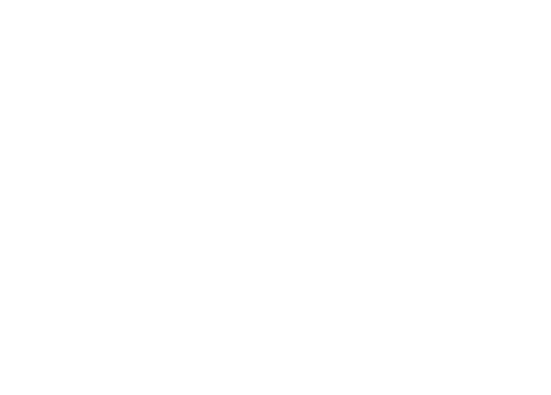
\includegraphics[width=0.7\textwidth]
    {./images/dummy.png}
  }
  \caption{Aufbau eines möglichen Videoanalysesystems}
  \label{messsystem}
\end{figure}

Die Kameras sollten in ihrer Ausrichtung und ihren Abbildungseigenschaften statisch sein. Setzt man dies voraus, besitzen die Kameras fest definierte Anordnungen zueinander. Die Auflösung des Kamerabilds muss ausreichend sein, um einzelne Personen aufzulösen. Nachdem das System aufgestellt und eingerichtet ist, müssen Grenzwerte der Messgrößen für jede Kamera erlernt und die Konfigurierung, wie in Abschnitt \ref{sec:konfig} beschrieben, durchgeführt werden. Das Eingangsbild der Kameras wird in rechteckige Bildausschnitte eingeteilt, für die jeweils Statistiken und Messwerte generiert werden. Diese werden als Listen oder Tabellen übertragen. In der Überwachungszentrale (siehe Abbildung \ref{messsystem}), in der die Datenströme der Kameras zusammengeführt werden, können, durch eine vorherige Kalibrierung, die Patch Positionen der Kamerabilder georegistriert auf Karten des Überwachungsgeländes übertragen werden. 
\newpage
Damit können zudem die Messungen aus Bildausschnitten verschiedener Kameras zusammengeführt und auf eine einzelne Ortsposition bezogen werden. Geben die Kameras als Netzwerk an einer Ortsposition eine durchschnittliche Messgröße in einem kritischen Bereich aus, können automatisch Notrufe und Warnungen ausgesendet werden. Zusätzlich kann das Personal in der Überwachungszentrale eine generierte Karte des Überwachungsgeländes, die georegistrierte und gemittelte Messungen der versch. Kameras darstellt, analysieren. Hier werden die durchschnittlichen Messwerte der verschiedenen Kameras als Heat Map wahlweise mit angezeigten Messwerten dargestellt. Zusätzlich kann im Nachhinein nach der Veranstaltung das Bewegungsverhalten der Personengruppen im Detail analysiert werden, indem Überwachungsvideos gespeichert werden und in Ruhe das Verhalten der Messgrößen betrachtet wird.
\newpage
Nachfolgend werden die Anforderungen des Systems an die Nutzer beschrieben:

\begin{flushleft}
\underline{Anforderungen des Systems:}
\end{flushleft}
\begin{itemize}
\item statische Rahmenbedingungen: statische Kameraperspektive
\item Kalibrierung der Positionen/Perspektiven der Kameras (wird nicht im Rahmen dieser Arbeit behandelt)
\item Konfigurierung mit, für die Szene sinnvollen, Evaluations-Parametern wie Such- oder Abstands-Radius
\item Konfiguration mit intrinsischen und extrinsischen Kameraparametern zur Skalierung von Evaluations-/Filtereinstellungen und Extremwerten (\zb in Form einer Patch-Karte)
\item Trainieren von Grenzwerten, um relative Messwerte zu erhalten
\end{itemize}

\section{Signalverarbeitung}
\label{sec:sig}
Um innerhalb eines Bildes lokale, statistische Messergebnisse zu erhalten, wird das Eingangsbild zunächst in rechteckige Bildausschnitte (Patches) eingeteilt, deren Höhe und Breite im Konfigurationsdialog bestimmt werden können. Die Trajektorien werden dabei ausgewertet, um sie in die Bildausschnitte entsprechend einzugliedern und patchbezogene Messwerte zu erhalten. Dieses Verfahren stellt in dieser Arbeit die Grundlage für die Signalverarbeitung, also die Umsetzung der Eingangsgrößen in Messgrößen, dar. Die Laufvariable $j$ ist in diesem Kapitel konsistent ein Index für die Frames einer Eingangsbildfolge und indiziert dabei den aktuellen Frame. Die Laufvariablen $x,y$ indizieren eine Position im Eingangsbild. Diese müssen immer innerhalb des Wertebereichs $W(w,h)$ des Bildausschnitts liegen. Die nachfolgend beschriebenen Messgrößen werden in jedem neuen Frame $j$ aktualisiert, d.h. neu berechnet und in sogenannte Patch Maps eingetragen.

\subsection{Trajektorien}
Die Umsetzung der Eingangsgrößen (-bilder) in Messgrößen erfolgt in dieser Arbeit auf Basis von erstellten Trajektorien (wie in Kapitel \ref{chap:grund} Abschnitt \ref{sec:trajektorien} beschrieben). 
\newpage
Die Trajektorien können mit dem erstellten Softwaremodul als Linien gezeichnet werden. Die Erfassung solcher Trajektorien anhand einer künstlich generierten Bildsequenz erkennt man beispielhaft in Abbildung \ref{trajektorien}. 
\bigskip
\begin{figure}[H]
\centering
  \begin{minipage}{0.45\textwidth}
    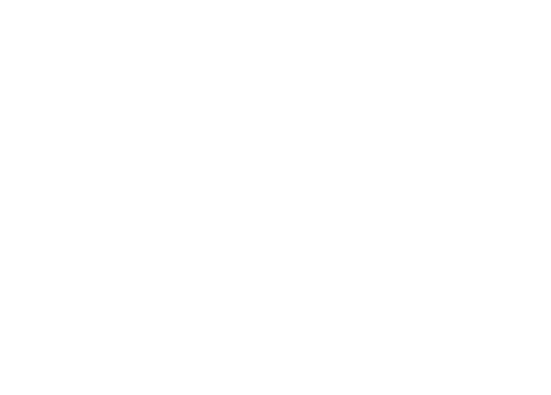
\includegraphics[width=\textwidth]{images/dummy.png}
    \label{a)}
  \end{minipage}
  \begin{minipage}{0.45\textwidth}
    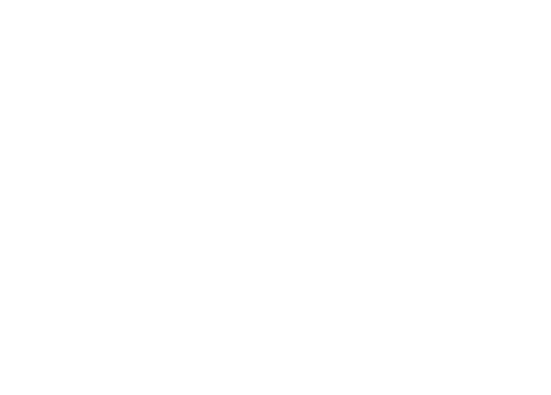
\includegraphics[width=\textwidth]{images/dummy.png}
    \label{b)}
  \end{minipage}
\caption{Erfassung und Darstellung von Trajektorien aus versch. Perspektiven \cite{CourtyPRL2014} \cite{Allain2012ICPR}}
\label{trajektorien}
\end{figure}

Hier erkennt man die automatische Erfassung von Trajektorien des entwickelten Verfahrens. Dabei werden 27 Frames einer künstlich generierten Bildsequenz analysiert, in der Personen, die anfangs in gleichem Abstand stehen, in alle Richtungen gegen die Wände drängen. Alle erfassten Koordinaten einer Trajektorie werden als zusammenhängende Linie in blau eingezeichnet. Nachfolgend erkennt man in Abbildung \ref{trajektorien_scenes} die Erfassung und Darstellung von Trajektorien in weiteren Szenen des verwendeten Datensatzes "`AGORASET''(siehe \cite{CourtyPRL2014} \cite{Allain2012ICPR}):
\bigskip
\begin{figure}[H]
\centering
  \begin{minipage}{0.45\textwidth}
    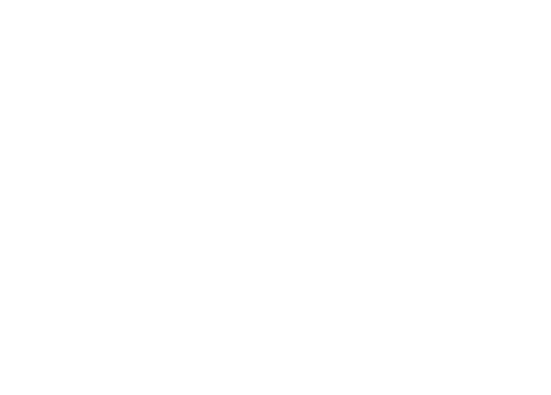
\includegraphics[width=\textwidth]{images/dummy.png}
    \label{a)}
  \end{minipage}
  \begin{minipage}{0.45\textwidth}
    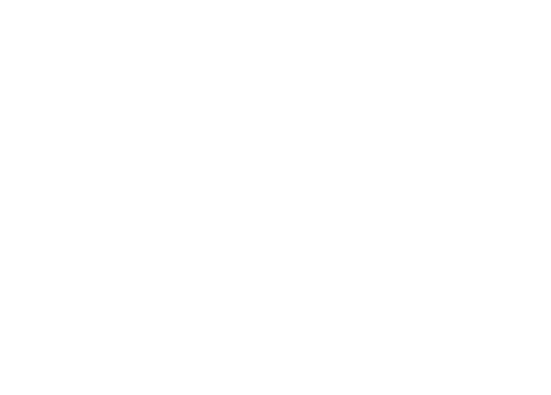
\includegraphics[width=\textwidth]{images/dummy.png}
    \label{b)}
  \end{minipage}
\caption{Erfassung und Darstellung von Trajektorien in diversen Szenarien \cite{CourtyPRL2014} \cite{Allain2012ICPR}}
\label{trajektorien_scenes}
\end{figure}

\newpage

\subsection{Personenzahl}
Die Zahl der bewegten Personen $N$ wird in ein Verhältnis mit der Summe an Trajektorienendpunkten (-spitzen) im Patch gesetzt. Um die Summe Dieser zu erhalten, wird die Kardinalität (Mächtigkeit) der Menge $S$ an Trajektorienspitzen (Trajektorien an ihrer Position im aktuellen Frame $j$), die sich innerhalb des betrachteten Bildausschnitts befinden, berechnet:

\begin{equation}
N = c_K\cdot |S| \hskip 30pt [\text{personen}]
\end{equation}
\vskip 5pt
\begin{flushleft}
für alle verwendeten Positionen $P(x,y)\in S$ gilt: $x,y\in W(w,h)$
\end{flushleft}
Hier bezeichnet $W(w,h)$ den zulässigen Wertebereich für die Bildkoordinaten $x,y$, falls diese sich im Bildausschnitt befinden. Dieser ist abhängig von der Breite $w$ und Höhe $h$ des Bildausschnitts.
%Damit werden nur die aktuellen Positionen der erstellten Pfade ausgewertet. Dazu wird die aktuelle (ggf. gefilterte) Trajektorienliste betrachtet und jede gefundene ID in einer neuen, mit 0 initialisierten Bildmatrix $S[x,y]$(Trajektorienspitzen) an ihrer aktuellen Position mit 1 markiert. Über Bewegungen $u,v$ vom Center Pixel an $x,y$ werden alle markierten Trajektorienspitzen, die sich im Bildausschnitt befinden, summiert.
%\begin{equation}
%N = C\cdot\sum_{u,v}{S[x+u,y+v]} \hskip 30pt [\text{personen}]
%\end{equation}
%mit $u,v \in W(u,v)$
\vskip 5pt

Wendet man auf $N$ einen zeitlichen gleitenden Mittelwert an, um Rauschen zu unterdrücken, erhält man die mittlere Personenzahl $\bar{N}_j$:

\begin{equation}
\bar{N}_j = \frac{1}{m}\sum_{i=0}^{m-1}{N_{j-i}} \hskip 30pt [\text{personen}]
\end{equation}
\vskip 10pt
Um relative Messgrößen zu erhalten, kann, im Laufe einer Testsequenz, ein Maximalwert $N_{max}$ für die (gemittelte) Personenzählung trainiert werden, der anschließend gespeichert wird. Die relative Personenzahl $N_{rel}$ ergibt sich somit zu:

\begin{equation}
    N_{rel}=\frac{\bar{N}_j}{N_{max}} \hskip 30pt [\%]
\end{equation}
mit $N_{rel}\in \{0..1\}$
\vskip 10pt
Ist dieser Maximalwert von Hand in einem vollen Patch gezählt worden oder anderweitig genau bekannt, kann dieser absolut als $N_{abs}$ im Konfigurationsdialog zusätzlich eingetragen werden. Dann kann aus der relativen Personenzahl im Bildausschnitt näherungsweise ein manuell definierbarer Normierungsterm (Kalibrierung des Zählsystems) $N_{scal}$ in $[\text{personen}]$ berechnet werden: 

\begin{equation}
    N_{scal}=N_{rel}\cdot N_{abs} \hskip 30pt [\text{personen}]
\end{equation}
\vskip 10pt
Ist weiterhin die projezierte Fläche A des Bildausschnitts bekannt kann außerdem ein manuell definierbarer Normierungsterm für die Personendichte $D_{scal}$ in $[\frac{\text{personen}}{m^2}]$ abgeleitet werden:

\begin{equation}
    D_{scal}=\frac{N_{rel}\cdot N_{abs}}{A} \hskip 30pt [\frac{\text{personen}}{m^2}]
\end{equation}
\newpage
\subsection{Personenfluss}
Der Personenfluss wird als der mittlere Nettozufluss an Trajektorien in einem Patch über die letzten $p$ (Schrittweite) Frames definiert. Um in jedem Frame zu- oder abfließende Trajektorien zu erfassen, wird ein Fluss-Akkumulator $F_{acc}$ eingerichtet, der den Beitrag +1 für eine in den Patch Eintretende und den Beitrag -1 für eine aus dem Patch austretende Trajektorie erhält. Dazu wird in jedem Frame die Differenz der Kardinalität der Menge S an Trajektorienspitzen und der Kardinalität der Menge $K$ an Trajektorienknoten (Position der Trajektorien im vorherigen Frame $j-1$) im Patch gebildet und über $p$ Frames gemittelt.

%Dazu werden die Trajektorien der aktuellen (ggf. gefilterten) Trajektorienliste in einer neuen, mit 0 initialisierten Bildmatrix $K[x,y]$ an ihrer Position im vorherigen Frame mit 1 markiert(Trajektorienknoten). Trajektorienspitzen S inkrementieren den Fluss im Patch, die Trajektorienknoten K dekrementieren ihn. Damit ergibt sich im Fall einer Grenzüberschreitung einer Trajektorie ein Beitrag +1 im Zielpatch und ein Beitrag -1 im Ursprungspatch.

\begin{equation}
F_{acc} = c_K\cdot (|S| - |K|) \hskip 30pt [\frac{\text{personen}}{\text{frame}}]
\end{equation}
\vskip 5pt
\begin{flushleft}
für alle verwendeten Positionen $P(x,y)\in S\cup K$ gilt: $x,y\in W(w,h)$
\end{flushleft}
\vskip 3pt
Der mittlere Nettozufluss über die letzten $p$ Frames beträgt somit:

\begin{equation}
    F = \frac{1}{p}\sum_{i=0}^{p-1}F_{acc,j-i} \hskip 30pt [\frac{\text{personen}}{\text{frame}}]
\end{equation}
\vskip 10pt
Wendet man auf $F$ einen zeitlichen gleitenden Mittelwert über M Frames an, um Rauschen zu unterdrücken, erhält man den mittleren Personenfluss $\bar{F_j}$.

\begin{equation}
\bar{F}_j = \frac{1}{m}\sum_{i=0}^{m-1}F_{j-i} \hskip 30pt [\frac{\text{personen}}{\text{frame}}]
\end{equation}
\vskip 10pt
Wird ein betragliches Maximum $F_{max}$ dieses mittleren Personenflusses algorithmisch gelernt, kann ein relativer Fluss angegeben werden:

\begin{equation}
F_{rel} = \frac{\bar{F}_j}{F_{max}} \hskip 30pt [\%]
\end{equation}
mit $F_{rel}\in \{0..1\}$
\vskip 10pt
Analog zur Personenzahl kann bei Bekanntheit von $N_{abs}$ ein manuell definierbarer Normierungsterm für den Personenfluss erhalten werden:
\vskip 5pt
\begin{equation}
    \bar{F}_{scal} = \bar{F}_j \cdot \frac{N_{abs}}{N_{max}} \hskip 30pt [\frac{\text{personen}}{\text{frame}}]
\end{equation}

\newpage
\subsection{Dynamik}
Zur Ableitung eines aussagekräftigen Dichtefaktors wird zusätzlich zur Personenzahl eine Kennzahl benötigt, die die vorherrschende Dynamik im Patch beschreibt. Dazu wird eine mittlere Merkmalsgeschwindigkeit im Patch eingeführt. Es wird erneut die Menge $S$ an Trajektorien betrachtet, deren Spitzen (aktuelle Positionen) sich innerhalb des Bildausschnitts befinden. Es werden Vektorbeträge für jede dieser Trajektorien nach folgendem Prinzip berechnet, um die Bewegungen über die letzten $q$ (Schrittweite) Frames zu erfassen. Im Fall, dass eine betrachtete Trajektorie noch keine $q$ Frames existiert, wird die Trajektorie aussortiert:
\begin{align}
\text{für} j-q \geq 0&: \hskip 10pt \abs{\vec{b_j}}(x,y) = \sqrt{[P_{j}(x) - P_{j-q}(x)]^2 + [P_{j}(y) - P_{j-q}(y)]^2} \notag \\
\text{sonst}:
\end{align}
\begin{flushleft}
für alle verwendeten Positionen $P(x,y)\in S$ gilt: $x,y\in W(w,h)$\vskip 5pt
Hier bezeichnet $P_j(x)$ die x-Position der Trajektorienspitze im aktuellen Frame j. $P_{j-q}(x)$ bezeichnet die x-Position der Trajektorienspitze vor $q$ Frames.
\end{flushleft} \vskip 5pt
Die mittlere Merkmalsgeschwindigkeit $B_j$ eines Bildausschnitts erhält man nun durch Mittelung über alle Vektorlängen $\abs{\vec{b}}_j(x,y)$ innerhalb des Patchs:

%\begin{equation}
%B_j = \frac{1}{|Z|}\sum_{u,v}\abs{\vec{b}}_j(x+u,y+v) \hskip 30pt [\frac{\text{px}}{q\cdot \text{frame}}]
%end{equation}
\begin{equation}
B_j = \frac{1}{|Z|}\sum_{k=0}Z_k \hskip 30pt [\frac{\text{px}}{q\cdot \text{frame}}]
\end{equation}

\begin{flushleft}
für alle verwendeten Vektorlängen $\abs{\vec{b}}_j(x,y)\in Z$ gilt: $x,y\in W(w,h)$.\vskip 5pt
Hier beschreibt $Z$ die Menge der berechneten Vektorlängen $\abs{\vec{b_j}}(x,y)$.\vskip 5pt
Um Rauschen zu unterdrücken, wird diese Kennzahl noch zeitlich gemittelt:
\end{flushleft}
\begin{equation}
\bar{B}_j = \frac{1}{m}\sum_{i=0}^{m-1}B_{j-i} \hskip 30pt [\frac{\text{px}}{q\cdot \text{frame}}]
\end{equation}
\vskip 5pt
Bei längerer Beobachtung der mittleren Merkmalsgeschwindigkeit in einer Testsequenz wird deutlich, dass sie in einem nicht vollgestauten (also unkritischen) Bildausschnitt immer oberhalb eines Schwellwertes liegt (nach Einschwingen des Systems). Dieser Schwellwert kann festgelegt werden, indem \zb ein Bildausschnitt betrachtet wird, der stetig vollgestaut wird und damit eine abnehmende mittlere Merkmalsgeschwindigkeit aufweist. Der Benutzer liest diese Messgröße, kurz nachdem er die Situation als kritisch einstuft, ab und trägt sie als Schwellwert $B_S$ ein. Der Schwellwert sollte, sobald kein Zu-/Abfluss in/aus dem Patch mehr existiert, schnell erreicht werden. Mit der Festlegung des Schwellwerts kann nun eine relative mittlere Merkmalsgeschwindigkeit $B_{rel}$ berechnet werden:
\newpage
\begin{equation}
    B_{rel}=\frac{B_S}{\bar{B}_j} \hskip 30pt [\%]
\end{equation}
mit: $B_{rel}\in \{0..1\}$
\vskip 10pt
Der Trägheitsfaktor $B_{rel}$ ist eine Art Staufaktor, der hohe Werte für geringe Dynamiken im Patch annimmt. Eine kritische Situation, wie beispielsweise ein Stau, liegt aber nur dann wirklich vor, wenn sich viele Personen im Bildausschnitt befinden und eine geringe Dynamik in Kombination vorliegt.

\subsection{Dichtefaktor}
Schlussendlich kann aus den zuvor abgeleiteten Größen ein Dichtefaktor definiert werden, der nur auf hohe Personenzahlen und hohe Trägheit in Kombination reagiert und hohe Werte annimmt.\vskip 5pt
\begin{equation}
\text{dFactor} = N_{rel}\cdot B_{rel} \hskip 30pt [\%]
\end{equation}
mit: $\text{dFactor}\in \{0..1\}$
\vskip 10pt

Der definierte Dichtefaktor funktioniert nur dann zuverlässig, wenn die Auflösung hoch genug ist, um Trajektorien von vereinzelten Personen zu erstellen. Treten Personengruppen hingegen nur noch als Anhäufung gleich heller Pixel auf, sind die Personen nicht separat erkennbar und die Personenzählung wird immer zu niedrig ausfallen, wobei gleiches für den Dichtefaktor gilt. Dieser Dichtefaktor macht weniger eine Aussage über eine Dichte in $[\frac{\text{personen}}{m^2}]$ als über den aktuellen Grad der Gefährdung der Besucher im betrachteten Bildausschnitt. Denn für hohe Dichtefaktoren, die kritischen Situationen entsprechen, ist sowohl die Personenzahl als auch die Trägheit im Patch hoch.

\subsection{Darstellung der Messgrößen - Aufbereitung}
Das Eingangsbild wird vom implementierten Verfahren wahlweise mit angezeigten Messwerten und eingezeichneten Bildausschnitten manipuliert. Außerdem können Messgrößen für einen genaueren Überblick durch Heat Maps dargestellt werden. Heat Maps sind farbkodierte Karten (ähnlich einer Wärmeverteilungskarte). Dabei wird das Bild zunächst in ein Grauwertbild konvertiert, damit es selbst keine Farbinformation mehr enthält. Dann wird für jeden Pixel eine neue Farbe im HSV-Farbraum bestimmt. Im HSV (hue, saturation, value)-Farbmodell kann der berechntete Grauwert an der Pixelposition als Helligkeitswert value eingesetzt werden, während die Farbsättigung (saturation) auf den Maximalwert gesetzt wird. Der Farbton (hue) wird dann auf den Wertebereich einer Messgröße skaliert und je nach Betrag färbt sich der Bildausschnitt mit zunehmender Messgröße von cyanblau bis dunkelrot. Zur Skalierung der Messgröße ist ein Training mit einer Testsequenz erforderlich. Dabei werden Maximal-/Minimalwerte der Messgröße vom Verfahren erlernt.
\newpage
Diese können in Konfigurationsdateien gespeichert und wiederverwendet werden. Hier wurde der gemessene Dichtefaktor zunächst auf einen Wertebereich von ${0..1}$ und anschließend auf dem Farbenkreis auf die Farben von Cyanblau bis Dunkelrot skaliert. Im HSV-Farbmodell entspricht dies einem zahlenmäßigen Farbton von 180-359. Formelmäßig kann man den Farbton hue so ausdrücken, falls $X_{rel}$ allgemein eine relative Messgröße beschreibt: 

\begin{equation}
    \text{hue} = X_{rel}\cdot(359-180) + 180
\end{equation}
\vskip 10pt
Ein Beispiel für die Darstellung einer Heat Map erkennt man in Abbildung \ref{heatmap}:
\vskip 10pt
\begin{figure}[h]
  \centering
  \fbox{
    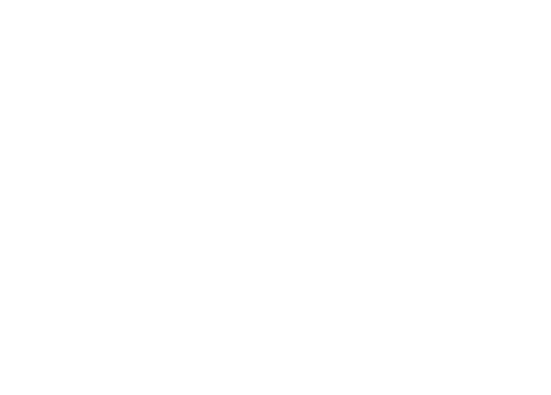
\includegraphics[width=0.8\textwidth]
    {images/dummy.png}
  }
  \caption{Darstellung des Dichtefaktors als Heat Map \cite{CourtyPRL2014} \cite{Allain2012ICPR}}
  \label{heatmap}
\end{figure}

Weil der Dichtefaktor aus der relativen Personenzählung und dem relativen Trägheitsfaktor abgeleitet wird, kann er nur für hohe Personenzahlen hohe Werte annehmen. Die maximale Personenzahl wird vom Verfahren in einer Lernphase statistisch geschätzt und tritt somit nur in einem voll befüllten Patch auf. Der abgeleitete Dichtefaktor beschreibt die Dichte der Personen im Bezug zur Fläche des Bildausschnitts. Personen, die zwar dicht aneinander stehen (siehe Abbildung \ref{heatmap} - lila), jedoch den Bildausschnitt nicht ausfüllen, erhalten keinen hohen Dichtefaktor. In einem solchen Fall würden aber in einem realen Szenario die Menschen sich instinktiv innerhalb des Bildausschnitts verteilen, weswegen eine Erkennung einer solchen Situation auch unerwünscht wäre.
\newpage
Nur im Fall einer hohen Personenzahl und zusätzlich hoher Trägheit im Patch nimmt der Dichtefaktor hohe Werte an, wie in Abbildung \ref{heatmap} im dunkelrot gefärbten Bildausschnitt zu erkennen ist. Ist die Erkennung von kleineren, dicht gedrängten Personengruppen erwünscht, können die Bildausschnitte auch verkleinert werden, damit weniger Personen den Bildausschnitt bereits ausfüllen. Dies birgt allerdings die Gefahr für häufige Fehlalarme.

\section{Konfigurierung}
\label{sec:konfig}
Der folgende Abschnitt befasst sich mit geplanten Ablaufschritten zur Konfigurierung des erstellten Softwaremoduls. Für optimale Ausnutzung des Funktionsumfangs müssen Grenzwerte geschätzt, Kameraparameter geladen, sowie Evaluations-, Filter- und Darstellungseinstellungen vorgenommen werden. Die Konfigurierung muss für jede Kamera/Sequenz einmal vorgenommen werden und kann dann gespeichert und wiederverwendet werden. Der Konfigurationsdialog des Softwaremoduls ist in Abb. \ref{konfig} dargestellt
\vskip 10pt
\begin{figure}[h]
  \centering
  \fbox{
    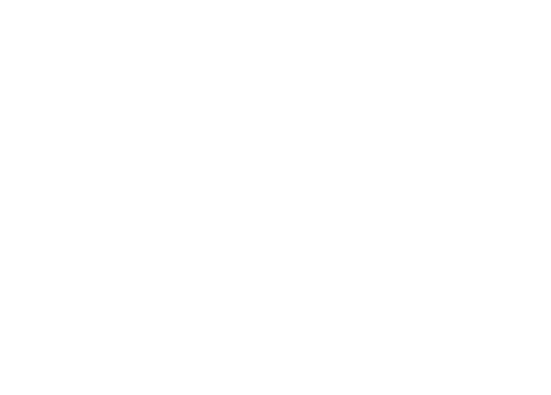
\includegraphics[width=0.65\textwidth]
    {images/dummy.png}
  }
  \caption{Konfigurationsdialog des Softwaremoduls}
  \label{konfig}
\end{figure}

%\subsection{Plugin: OCV\_Corner Tracker}
%Der vorgeschaltene Corner Tracker, wie in Kapitel \ref{chap:grund} Abschnitt \ref{sec:trajektorien} beschrieben, muss zunächst konfiguriert werden. Dazu wird das Ausgangsbild dieses Plugins betrachtet, in dem die Detektionen des Harris Corner Detectors als Punkte eingezeichnet werden können. Die Einstellung "`maxCorners'', die die maximale Anzahl an detektierten Ecken angibt, wird idealerweise auf einen hohen Wert gesetzt(\zb $10000$). Nun wird das "`QualityLevel'', das die minimale Qualität der detektierten Ecken angibt, stetig vermindert, bis die im Bild zu sehenden Personen im Durchschnitt mindestens eine Eckendetektion/Person erhalten. Dieses Quality Level wird eingestellt und nicht mehr verändert, solange keine neue Szene verwendet wird.

\subsection{Patch-Map Dimension}
Um die Patch Maps den Wünschen des Anwenders anzupassen, kann Höhe und Breite eines Bildausschnitts im Konfigurationsdialog gewählt werden. Anschließend muss das aktuelle Bild nach dem Betätigen eines Reset-Button neu geladen werden, um die Änderungen zu aktualisieren. Passen die gewählten Patches nicht gradzahlig ins Ausgangsbild, werden über den Rand überlappende Bildausschnitte am Rand erstellt. Wie bereits in Abschnitt \ref{sec:sig} erwähnt, können die Patches wahlweise aufbereitet mit Messwerten oder Heat Maps eingezeichnet werden. Dieses aufbereitete Ausgangsbild wird vom Nutzer schließlich vereinfacht analysiert.

\subsection{Geschwindigkeitsschwelle}
Zur angepassten Unterscheidung von statischen Merkmalen zu Bewegten, wird eine konfigurierbare Geschwindigkeitsschwelle in $[\frac{\text{px}}{\text{frame}}]$ festgelegt. Zur Verwaltung (d.h. Erstellung und Fortführung) von Trajektorien werden nur Merkmale betrachtet, die oberhalb dieser festgelegten Geschwindigkeitsschwelle liegen. Statische Merkmale wie Ecken von Häusern oder Gegenständen werden somit weitgehend gefiltert, jedoch auch statische Personen. Eine geeignete Geschwindigkeitsschwelle erhält man empirisch, indem man zunächst den Suchradius vorübergehend auf $0$ setzt, um ein Verknüpfen der Trajektorien weitgehend zu verhindern. So entstehen ständig neue Trajektorien an detektierten Ecken von Personen ohne unberechenbare Verknüpfungen. Anschließend vermindert man die Geschwindigkeitsschwelle stetig und lässt sich die Spitzen (aktuelle Positionen) der Trajektorien in der laufenden Bildsequenz einzeichnen. Die bewegten Personen im Bild sollten im Durchschnitt mindestens eine Trajektorie pro Person erhalten. Die höchste Geschwindigkeitsschwelle für die dies zutrifft, wird eingestellt.

\subsection{Maximale Verweilzeit}
Um zu erlauben, dass Trajektorien für eine gewisse Frame-Dauer statisch auf ihrer Position verharren, wird eine maximale Verweilzeit in $[\text{frame}]$ gewählt. Dazu wird bestimmt, ob in der Umgebung einer Trajektorien-ID Merkmale oberhalb der Geschwindigkeitsschwelle liegen. Wenn ja, ist diese Trajektorie redundant, weil die Trajektorie fortgeführt wird. Wird kein solches Merkmal gefunden, kann die Trajektorie nicht fortgeführt werden und die Position der ID wird in einer Matrix (Stop-and-Go-Map) mit der Bildgröße inkrementiert, sofern der Wert die maximale Verweilzeit noch nicht erreicht hat. Sollte die Toleranz bereits erreicht sein, wird die Position in der Stop-And-Go-Map zurück auf 0 gesetzt und die Trajektorie entfernt.

\newpage

\subsection{Mittelungsdistanz}
Wie in Abschnitt \ref{sec:sig} behandelt, werden zeitliche Mittelungen im entwickelten Verfahren als gleitender Mittelwertfilter ausgeführt. Dazu kann im Konfigurationsdialog eine Mittelungsdistanz $m$ festgelegt werden, die die Ordnung des Filters angibt, also über wieviele Frames der Mittelwertfilter ausgeführt wird. Meist eignet sich eine Mittelungsdistanz von $10-20$ Frames, um Rauschen weitgehend zu unterdrücken.

\subsection{Suchradius}
Wie bereits in Kapitel \ref{chap:grund} Abschnitt \ref{sec:trajektorien} behandelt, werden nur gefundene Merkmale, die oberhalb der Geschwindigkeitsschwelle liegen, behandelt. Wird ein Merkmal in der Umgebung einer ID in der ID Map gefunden, wird diese, bereits vorhandene, Trajektorie mit dem gefundenen Merkmal verknüpft und fortgeführt. Zur Suche nach Merkmalen in der Nachbarschaft ist die Definition eines Suchradius in $[\text{px}]$ nötig, innerhalb dessen eine Suche nach Merkmalen/IDs vorgenommen wird. Dieser kann global im Konfigurationsdialog festgelegt werden. Einen geeigneten Suchradius für die Merkmale erhält man empirisch, indem man zunächst beim kleinsten Wert (1) beginnt und sich die Trajektorien, nach gewisser Dauer, in einem bestimmten Frame der Testsequenz einzeichnen lässt. Dies wiederholt man mit steigenden Radien, bis man durchgängige, lange Pfade erkennen kann. Der niedrigste Radius für den dies zutrifft, wird als Suchradius gewählt. Mit weiter steigenden Radien erscheinen die Pfade als eckiger/zackiger, weil die Merkmale großzügiger mit den ID's verknüpft werden. Damit ergibt sich eine höhere Toleranz für weit von der ID entfernte Merkmale, die möglicherweise schon zu einer anderen Person gehören und damit ein individuelles Tracking maßgeblich erschweren. Wechselt eine Trajektorie zwischen verschiedenen Personen, entstehen dabei Zacken. Gezeichnete Trajektorien werden in Abbildung \ref{trajektorien_drawn} für verschiedene Suchradien dargestellt.

\newpage
\begin{figure}[h]
\centering
    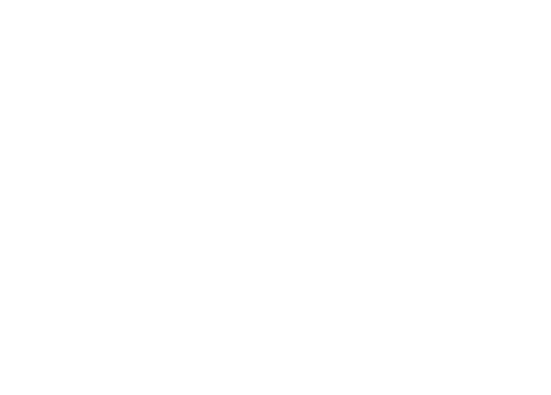
\includegraphics[width=0.49\textwidth]{images/dummy.png}
    a) $r=1$

    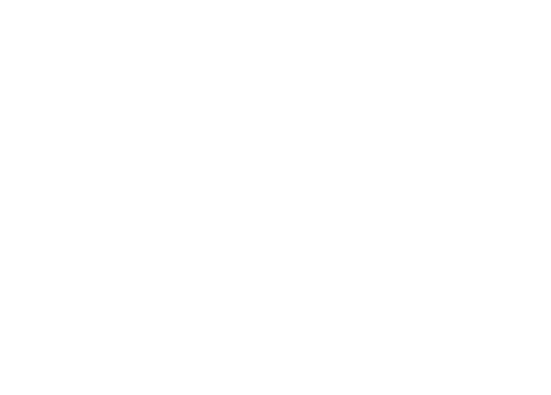
\includegraphics[width=0.49\textwidth]{images/dummy.png}
    b) $r=2$

    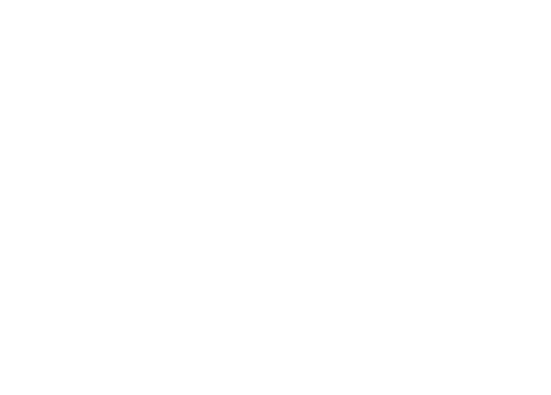
\includegraphics[width=0.49\textwidth]{images/dummy.png}
    c) $r=5$
    
\caption{Gezeichnete Trajektorien für versch. Suchradien}
\label{trajektorien_drawn}
\end{figure}
\newpage

Man erkennt hier, dass für kleinere Radien (siehe a)) die Trajektorien fragmentiert wirken. Erhöht man den Radius (vgl. b)), funktioniert das Verknüpfen der Pfade zuverlässiger und man erkennt durchgängige Trajektorien. Wird der Radius wie in c) noch weiter erhöht, entstehen Zacken in den Pfaden, weil die Trajektorien großzügiger verknüpft werden und eine höhere Toleranz für Merkmale gesetzt wird, die von der ID weit entfernt liegen. Hier wurde der Radius 2 als Suchradius gewählt und gespeichert.

\subsection{Abstands-Radius}
Ebenso wie es zu vermeiden gilt, dass eine Trajektorie zwischen verschiedenen Personen wechselt, gilt es zu vermeiden, dass im zeitlichen Verlauf der Eingangssequenz im Durchschnitt unterschiedlich viele Trajektorien pro Person geführt werden. Dazu wird ein Abstands-Radius eingeführt, innerhalb dessen, nach der Evaluation eines Frames, die Nachbarschaft in der ID Map nach anderen IDs abgesucht wird. Wird eine ID gefunden, wird die länger bereits vorhandene Trajektorie behalten und die Kürzere entfernt, sofern ein Unterschied besteht. Damit unterdrückt man neue, kurze Trajektorien, die durch Rauschen entstehen und sorgt zudem dafür, dass die Trajektorien und damit auch die detektierten Personen zusammen eine große Fläche einnehmen müssen, um eine hohe Zahl an Trajektorien zu ermöglichen. Dies ist erwünscht, weil sonst beliebig viele Trajektorien an einer Person entstehen können, auch wenn diese alleine keine große Fläche einnimmt, was zu einer zu hohen Personenzählung führt. Eine große Zahl an Personen nimmt eine große Bildfläche ein und infolgedessen sollten auch nur in diesem Fall viele Trajektorien erlaubt sein. Durch Einführung des Abstands-Radius vermindert man Probleme, die durch gegenseitige Verdeckung der Personen entstehen. In weniger dichten Gebieten nimmt eine Person in der Regel eine größere Fläche ein, weil sie nicht durch andere Personen verdeckt wird. So können allerdings auch mehr Trajektorien an dieser Person entstehen, weil mehr Kanten dieser Person sichtbar sind. Nimmt die Personendichte an diesem Ort im Verlauf der Bildsequenz zu, wird diese Person mehr und mehr von Anderen verdeckt und es entstehen im Durchschnitt weniger Trajektorien pro Person, weswegen trotz der deutlich erhöhten Personenzahl, etwa die gleiche Zahl an Trajektorien und damit die gleiche Personenzählung wie zuvor vorliegt. Führt man einen Abstands-Radius ein, können nur bedingt viele Trajektorien an der unbedeckten Person entstehen und die Zahl an Trajektorien pro Person ist sowohl im Zustand geringer als auch hoher Personendichte in etwa gleich, wobei sich im Zustand hoher Dichte folglich, wie gewünscht, eine deutlich erhöhte Personenzählung ergibt.

\subsection{Ortsbezogener Ausgleich}
Bei Einführung dieses Abstands-Radius muss bedacht werden, dass die Ursprungsorte der Pixel im Eingangsbild, je nach Perspektive, unterschiedliche Abstände zum Kameraobjektiv aufweisen. Dieser Effekt wirkt sich umso stärker aus, je weiter man von der Vogelperspektive (Draufsichtperspektive) abweicht. 
\newpage
Demnach ist der Pixelabstand $d(x,y)$ in $[\frac{m}{\text{px}}]$ in entfernteren Bildregionen höher, weil solche Bildregionen kleiner skaliert abgebildet sind. Dies wird in Abblidung \ref{Skalierung} verdeutlicht:
\vskip 10pt
\begin{figure}[h]
  \centering
  \fbox{
    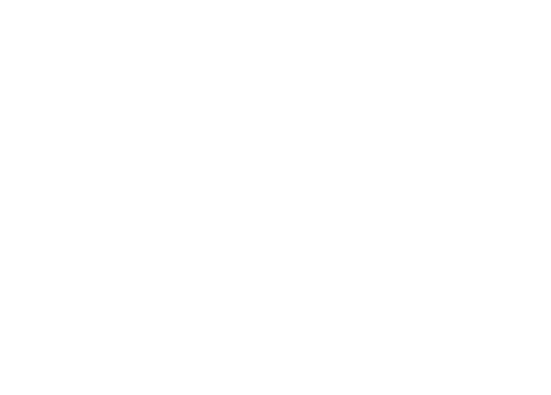
\includegraphics[width=0.6\textwidth]
    {images/dummy.png}
  }
  \caption{versch. Bildregionen mit unterschdl. Abständen zum Kameraobjektiv}
  \label{Skalierung}
\end{figure}

Deshalb sind Menschen in weiter entfernten Bildregionen auch weniger Pixel hoch und voneinander entfernt. Sie nehmen damit, bei gleichbleibender Personenzahl, eine geringere Bildfläche ein, wobei weniger Trajektorien pro Person erfasst werden, weil die Kantenlänge in $[\text{px}]$ verringert ist. Der Abstands-Radius sollte demnach in entfernteren Bildregionen sehr klein sein, um die ohnehin schon geringe Zahl an Trajektorien pro Person nicht weiter zu verringern. Dieser kleinste Abstands-Radius kann im Konfigurationsdialog festgelegt werden. Je näher sich das Objekt an der Kamera befindet, desto größer wird es abgebildet und der Abstands-Radius sollte mit einem entsprechenden (nichtlinearen) Skalierungfaktor vergrößert werden. Infolgedessen sollte idealerweise eine Skalierungsfunktion in Form einer Bildmatrix vorliegen, in der der Pixelabstand (die Skalierung) in $\frac{m}{\text{px}}$ relativ zum größten Pixelabstand (zur kleinsten Abbildung) in $\frac{m}{\text{px}}$ im Eingangsbild für alle Bildkoordinaten $x,y$ eingetragen ist. Mit Skalierungsfunktionen können Abstands-Radius oder andere Evaluations- und Filtereinstellungen sowie Grenzwerte skaliert werden. Eine solche Skalierungsfunktion kann leicht aus einer vollständig dokumentierten Kamerakalibrierung generiert werden. Alternativ kann auch eine Abstands-Radius Karte erlernt werden. Dazu muss der Abstands-Radius in $\text{px}$ am unteren und oberen Bildrand als größter und kleinster Radius eingesetzt werden. Die Pixel zwischen oberer und unterer Bildzeile erhalten interpolierte Abstands-Radien zwischen den beiden Vorgegebenen. Dabei wird davon ausgegangen, dass die Entfernung vom Kameraobjektiv vom Unteren zum oberen Bildrand hin zunimmt, was oft in guter Näherung zutrifft. Wird keine Abstands-Radius-Karte vorgegeben wird der kleinste Abstands-Radius global verwendet. Für den kleinsten Abstands-Radius kann die Personenhöhe (in $\text{px}$) für den maximal zulässigen Abstand von Person zu Kamera eingesetzt werden (minimale Auflösung einer Person).
\newpage
Alternativ kann auch eine geometrische Kalibrierung vorgenommen werden, um den Einfluss der unterschiedlichen Abstände der Bildregionen vom Kameraobjektiv zu verringern. Dazu werden bestimmte Bildregionen neu skaliert, so dass ursprünglich größer skalierte Gebiete, in denen also eine Person mit deutlich mehr Pixeln aufgelöst wird, eine geringere Auflösung erhalten, als Gebiete in denen die Personen ohnehin schon klein skaliert sind. Dabei verzerrt sich das Bild geometrisch. Da nun in allen Bildregionen eine Person mit näherungsweise gleich vielen Pixeln aufgelöst wird, werden nun Inhomogenitäten in der durchschnittlichen Zahl an Trajektorien pro Person vermieden. Dies wird in Abbildung \ref{geokal} dargestellt:

\begin{figure}[H]
\centering
  \begin{minipage}{0.45\textwidth}
    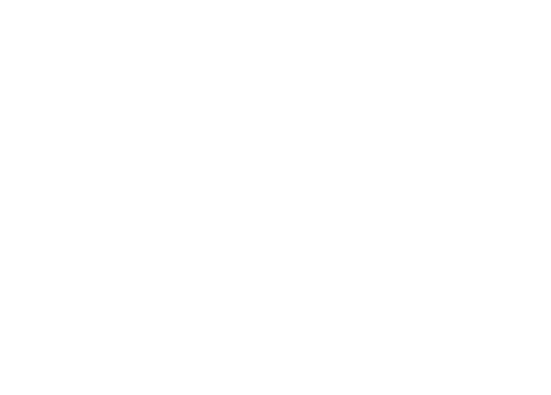
\includegraphics[width=\textwidth]{images/dummy.png}
  \end{minipage}
  \begin{minipage}{0.45\textwidth}
    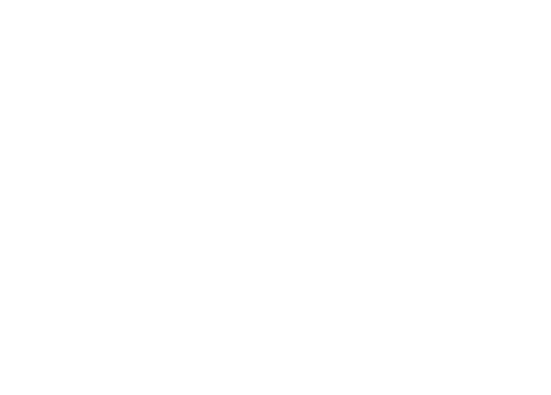
\includegraphics[width=\textwidth]{images/dummy.png}
  \end{minipage}
\caption{Verfahren: geometrische Kalibrierung}
\label{geokal}
\end{figure}


\subsection{Distanzschätzung}
Sind Aperturwinkel $\omega$, Tilt-Winkel $T$, sowie die Höhe $h$ der Kamera bekannt, lassen sich näherungsweise die Abstände der Ursprungsorte von oberer und unterer Bildzeile vom Kameraobjektiv bestimmen. Dazu betrachtet man folgende Skizze in Abbildung \ref{distanz}:

\begin{figure}[h]
  \centering
  \fbox{
    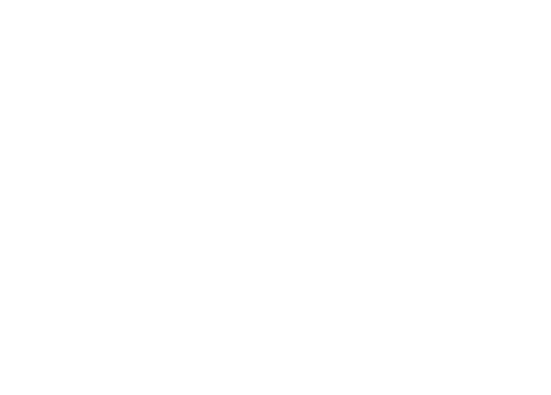
\includegraphics[width=0.6\textwidth]
    {images/dummy.png}
  }
  \caption{Distanzschätzung der Bildzeilen}
  \label{distanz}
\end{figure}

Wendet man die trigonometrischen Gesetze an, wird hierbei deutlich:
\begin{align}
    d_1 &\approx \frac{h}{\sin{(T + \frac{\omega}{2})}} \notag \\
    d_2 &\approx \frac{h}{\sin{(T - \frac{\omega}{2}})}
\end{align}

Die Abstände der Ursrpungsorte von oberer und unterer Bildzeile vom Objektiv können mit diesen Formeln näherungsweise berechnet werden. Um eine Patch Map zu erhalten, die genäherte Distanzen der Bildauschnitte enthält, wird die Distanz zeilenweise zwischen oberer und unterer Bildzeile interpoliert und innerhalb der Patches gemittelt. 

Liegt eine vollständig dokumentierte Kamerakalibrierung vor, ist dieses Verfahren redundant, weil aus der Kalibrierung der Abstand jedes Ursprungsorts im Eingangsbild berechnet werden kann. Dies ist jedoch für die Bilddaten, die für diese Arbeit vorliegen, nicht gegeben.

%\subsection{Trainieren von Extremwerten}
%Um relative Messgrößen zu erhalten, müssen Extremwerte von bestimmten Messgrößen trainiert werden. Relative Messungen sind nötig, um Angaben in $\%$ zu erhalten und damit Skalierungen der Messgrößen beispielsweise auf den Farbbereich von Heat Maps vornehmen zu können. Nach aktuellem Stand können diese Extremwerte automatisch trainiert werden:

%\begin{itemize}
    %\item Maximum der Personenzählung
    %\item Maximum/Minimum des Personenflusses
    %\item Maximum des Dichtefaktors
%\end{itemize}

%Zum Trainieren der Extremwerte können Frame Intervalle(\zb $0-50$) festgelegt werden, innerhalb derer das Training vorgenommen wird.

%Alternativ können diese Extremwerte auch im Konfigurationsdialog eingetragen werden, falls diese schon bekannt sind. Der Schwellwert der mittleren Merkmalsgeschwindigkeit über die letzten 10 Frames muss manuell eingetragen werden und wird meist aus dem Verhalten der Messgröße erschlossen. 
%\newpage
%Idealerweise sollten Patch Maps vorliegen oder generiert werden, in denen Extremwerte für jede Messgröße skaliert auf jeden Bildausschnitt eingetragen sind. Die Extremwerte für Personenzahl und andere Messgrößen sowie Evaluations- und Filtereinstellungen sollten über das Eingangsbild hinweg örtlich variieren. Eine klein skalierte Bildregion enthält beispielsweise klein skalierte Personen, weswegen sich auch viele Personen gleichzeitig in ihr befinden können. In einer größer skalierten Bildregion sind auch die Personen größer skaliert und es passen insgesamt weniger Personen in diesen Bildausschnitt. Die Skalierung der Extremwerte auf die verschieden weit entfernten Bildausschnitte kann mit der zuvor beschriebenen Karte, in der an jedem Ort $x,y$ der Pixelabstand relativ zum größten Pixelabstand im Eingangsbild eingetragen ist, durchgeführt werden.

%Nach dem Training/der Eingabe der Extremwerte können diese in Konfigurationsdateien gespeichert und wiederverwendet werden.

\subsection{Filtereinstellungen}
Leichte Kamerabewegungen lassen Trajektorien auch an Ecken von Gegenständen entstehen. Zusätzlich nehmen Wasser- und Windbewegungen (\zb Blätter) Einfluss. Diese Bewegungen sind meist klein, können aber dennoch die gewählte Geschwindigkeitsschwelle betragsmäßig überschreiten. Erwünscht sind jedoch nur Trajektorien an Personen. Um solche fälschlicherweise entstandenen Trajektorien zu entfernen, können, vor der Umsetzung in Messgrößen, Filter auf die Trajektorien angewandt werden.

Nachfolgend werden die implementierten Filter aufgezählt:

\begin{itemize}
    \item minimale Vektorlänge der Trajektorie über die letzten $m$ Frames$\Rightarrow$kleine Kreisbewegungen werden gefiltert, exzentrische, gestreckte Bewegungen werden behalten
    \item minimale Eintragslänge der Trajektorie$\Rightarrow$kurze Trajektorien werden gefiltert, robuste, lange Trajektorien werden behalten
    \item maximale Eintragslänge der Trajektorie$\Rightarrow$besonders lange Trajektorien werden gefiltert 
\end{itemize}

